\chapter{Objetivos y Metodología}
\label{cap:objetivos}
Tras haber presentado el contexto en el que se desarrollará este proyecto, en este capítulo se fijarán los objetivos y se expondrán los requisitos para llegar a la solución.
\section{Descripción del problema y requisitos}
\label{sec:descripciondelproblema}

El fondo oceánico es uno de los grandes misterios de la actualidad. La mayor parte del suelo oceánico no ha sido explorado, y eso supone un gran problema. Con este robot podremos rozar un poco este mundo submarino tan fascinante, e intentar descubrir algunas de las magníficas maravillas que esconde.

El robot contiene una cámara de alta resolución que permite visualizar el suelo oceánico. Cuando la visión de la cámara sea baja o nula, precisaremos de las luces y los láseres incorporados, con ellos, podremos visualizar mejor el entorno y saber la distancia a la que se encuentren los objetos, plantas o animales. 

Los requisitos indispensables para realizar el proyecto son:
\begin{enumerate}
\item \textbf{Impermeabilidad} durante todo el proceso de sumersión.
\item \textbf{Conectividad.} El robot puede alcanzar una distancia de 100 m sin que pierda señal.
\item \textbf{Duración de las baterías.} El robot debe permanecer activo durante 6 horas. 
\item \textbf{Web Cockpit.} Control del funcionamiento del robot.
\end{enumerate}

\section{Objetivo del proyecto}
\label{sec:objetivos}

El objetivo del proyecto es el montaje, configuración del software de ROV y ROS, y unas pruebas de campo del robot submarino OpenROV. 
\\Se montará de cero el robot submarino, utilizando los materiales dados por la comunidad de OpenROV. A la placa de OpenROV se le instalará un PLC para la comunicación del robot con el portátil y otra placa BeagleBone, que llevará implantado el software necesario para la comunicación y funcionamiento con el robot.
\\Además, se implantará una biblioteca de ROS dentro de OpenROV para que también se pueda comunicar a través del framework de robótica más famoso. Con esta biblioteca instalada y ejecutando el ROS Master en el portátil, se podrá realizar una comunicación.

\section{Metodología de desarrollo}
\label{sec:metodologiadedesarrollo}

En el desarrollo del sistema descrito, el modelo de ciclo de vida utilizado ha sido el modelo Modelo en cascada\cite{cascada}.

Es un proceso secuencial (como en una cascada de agua) en el que se definen las fases de: análisis de las necesidades, diseño, implantación, validación, integración y mantenimiento. 

Los principios básicos del modelo de cascada son los siguientes:
\begin{figure} [hbtp]
  \begin{center}
    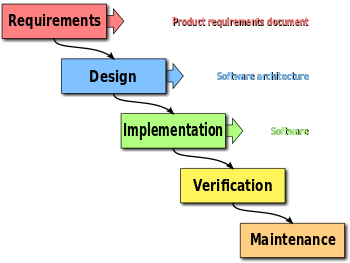
\includegraphics[width=11cm]{img/cap2/Waterfall_model}
  \end{center}
  \caption{Modelo en cascada.}
  \label{fig:Waterfall_model}
\end{figure}
\newpage

\section{Plan de trabajo}
\label{sec:plandetrabajo}

Para poder abordar el problema se han marcado una serie de objetivos a completar. Dichos hitos son los siguientes:

\begin{enumerate}
\item Estudio, comprensión y montaje del OpenROV 2.8.
\item Una vez terminado el montaje, se realizará la conexión del ROV para comunicarse con el portátil.
\item Fase de pruebas. Se probará el robot en distintos entornos para comprobar su funcionamiento.
\item Estudio y comprensión de los paquetes de ROS roslibjs\footnote{http://wiki.ros.org/roslibjs} (biblioteca de JavaScript para interactuar con ROS) y rosbridge\footnote{http://wiki.ros.org/rosbridge\_suite} (envía mensajes JSON para comunicarse con ROS a través de websocket, además controla la ejecución de los nodos).
\item Integración de ROS y OpenROV.
\end{enumerate}